\chapter{(OLD) Paper discussion \& conclusion (to be converted over)}

The question of what features of the world should be present in a `good' representation that improves the performance of an artificial agent for a variety of tasks is one of the key questions in representation learning.
The other key question in representation learning: `How do we build algorithms that produce representations with these features?' is beyond the scope of this work.

\autocite{Higgins2018} proposes that the symmetries of the world are important structures that should be present in an agent's representation of the world.
They formalise this proposal using group theory as SBDRL, which is made up of a disentangling condition that defines the disentangling of transformations as commutative subgroups and a group equivariant condition.
We take the proposal that the symmetries of the world are important structures that should be present in an agent's representation of the world one step further and propose that the relationships of transformations of the world due to the actions of the agent should be included in the agent's representation of the world and not just the actions of the agent that are symmetries.
To show that the relationships of transformations of the world due to the actions of the agent are important we set out a mathematical framework, in a similar vein to what \autocite{Higgins2018} does with SBDRL.
We then used this framework to derive and identify limitations in the SBDRL framework.
This has two benefits, (1) it shows that the framework we lay out encompasses the previous work (SBDRL) and how our framework encompasses it, and (2) it identifies worlds where the previous work cannot describe the relationships between the transformations of a world due to the actions of an agent.
We use algorithmic methods, newly designed by us for this work, to extract the algebras of the actions of an agent of some example worlds with transformations that cannot be fully described by SBDRL.
We decided to use worlds that exhibit features commonly found in reinforcement learning scenarios because representation learning methods are commonly used in reinforcement learning as representation learning has been shown to improve the learning efficiency, robustness, and generalisation ability of reinforcement learning algorithms, and so it is likely that this work will aid the construction of representation learning algorithms that will be used in the field of reinforcement learning.

Finally, we use category theory to generalise core ideas of SBDRs, specifically the equivariance condition and the disentangling definition, to a much larger class of worlds than previously with more complex action algebras, including those with irreversible actions.
In doing this we have managed to use our framework to derive and then generalise the core idea of SBDRL: the relationships between transformations due to the actions of the agent are important aspects of the world that should be included in the agent’s representation of the world.
We also propose that category theory appears to be a natural choice for the study of transformations of a world because category theory focuses on the transformation properties of objects and the perspective that the properties of objects are completely determined by their relationship to other objects is a key result of category theory (the Yoneda Lemma).

The framework we have set out and its results have much room for expansion in future work, including the following:
(1) How would we deal with transformations of the world that are not due to the actions of an agent?
Is it possible to decouple these transformations from the actions of the agent? Could the result of the agent's actions be estimated by taking some sort of average of the effect of performing each action across a diverse range of states or by working out external causal factors?
(2) How would partial observability affect the agent's representation?
(3) What effect would the use of continuous actions have?
The inclusion of continuous actions would not affect the generalisation of the equivariance condition or disentangling definition given in Section ref[sec:Generalising SBDRL]; there would just be additional conditions on the equivariance conditions to preserve continuity.
A potentially interesting line of research would be the following: if the reality is, as we have argued, that the agent’s representation is actually discrete due to the precision of the agent’s sensors, would this have any effect on the structure of the agent’s representation or the agent’s learning - similar to how the quantisation of particles has knock-on effects in quantum physics?
(4) What algebraic structures would be given by different equivalence relations?
For example, instead of an equivalence relation that equates two actions if they always produce the same result when acting on a world state, how about an equivalence relation that also requires that the number of minimum actions taken is the same up to $\textit{(number of minimum actions)} \text{mod} (2)$ for actions to be considered equivalent.
(5) Under what conditions can we disentangle reversible and irreversible actions?
(6) Could our category theory generalisation of the SBDRL equivariance condition also be used to describe other uses of equivariance conditions in AI, such as unifying the different equivariance conditions given by \autocite{Bronstein2021} through natural transforms?
(7) How can our framework be used to develop better representation learning algorithms?

While a focus on symmetries is becoming more prominent in representation learning, in this work we have sought to take some key results of mathematical frameworks based on symmetries and generalise them to encompass all transformations of the world due to the actions of an agent.
We hope the work presented here will stimulate further work in this direction, especially in the use of category theory as a natural tool to describe the transformations of a world.

\whendraft{
\noindent\rule{\textwidth}{1mm}
\begin{enumerate}
    \item Agent perception is always discrete because, even in a continuous world, there is always a limit to what an agent can perceive there exists two world states are indistinguishable to agent (\textit{e.g.}, the agent's sensors are not precise enough to distinguish between the two world states).
    
    \item Does treating the world as `effectively continuous' make a difference?
\end{enumerate}
}

%%%%%%%%%%%%%%%%%%%%%%%%%%%%%%%%%%%%%%%%%%%%%%%%%
% \chapter{(OLD) Paper discards (to convert over)}

\section{Reproducing SBDRL}

\subsection{SBDRL through equivalence}

%%%%%%%%%%%%%%%%%%%%%%%%%%%%%%%%%%%%%%%%%%%%%%%
\subsection{Equivalence of transitions}


\textbf{Notes:}
\begin{itemize}
    \item \textbf{
            [Removed this section because the link $l_{\sim}$ between $D_{A/\sim}$ and $A/\sim$ is not well defined - see notes in PhD Notebook 1 -, and only equivalence of actions is strictly required for the paper.]
            }
    \item \cite{Higgins2018} states that two transformations of the world are the same if they start in the same world state and end in the same world state [I think - check exact wording - actually appears that they just imply that actions are equivalent].
    They then use this to jump to a form of equivalence of actions.
    We know this jump cannot be made, and that the equivalence of actions must be defined separately (and that the desired definition of equivalence of actions is different from this definition of equivalence of transitions).
    Write this up in the thesis in an "Analysis of relevant literature" chapter as a flaw in the SBDRL framework proposed in \cite{Higgins2018}.
    The issue with the equivalence of observations being wrong in Hugo's Sensory action sequences paper can also go in the "Analysis of relevant literature" chapter.
\end{itemize}

We define an equivalence relation that allows us to treat transitions that start in the same world state and end in the same world state as being the same, and we define an equivalence relation that allows us to treat two actions as the same if their effects are the same if they are applied to a world state.

While not explicitly mentioned in \cite{Higgins2018}, a key assumption of \cite{Higgins2018}'s work is that two transformations of the world are the same if they start in the same world state and end in the same world state.
Therefore, we define an equivalence relation on the elements of $D$ that says that two transitions are equivalent if they share the same source and share the same target (see \hyperref[prp:w1-to-w2-equivalence]{proposition \ref*{prp:w1-to-w2-equivalence}} below).



\begin{definition}[Equivalence of transitions under $\sim$]
    We say that $d \sim d'$ if $s(d) = s(d')$ and $t(d) = t(d')$.
\end{definition}

\begin{proposition}\label{prp:w1-to-w2-equivalence}
    $\sim$ defines an equivalence relation on $D$.
\end{proposition}\begin{proof} 
    \textbf{Reflexive.}
    Since $s(d)=s(d)$ and $t(d)=t(d)$ for any $d \in D$, then $d \sim d$.
    
    \textbf{Transitive.}
    If $d \sim d'$ and $d' \sim d''$ for any $d, d', d'' \in D$, then $s(d) = s(d')$, $t(d) = t(d')$, $s(d')=s(d'')$, and $t(d')=t(d'')$.
    These four equations can be used to show that $s(d) = s(d'')$ and $t(d) = t(d'')$.
    This is the condition for $d \sim d''$.
    
    \textbf{Symmetric.}
    If $d \sim d'$, then $s(d)=s(d')$ and $t(d)=t(d')$ hence $d' \sim d$.
\end{proof}

We define the canonical projection map $\pi_{D}: D \to D/\sim$ that sends transitions in $D$ to their equivalence classes under $\sim$ in the set $D/\sim$.
We denote the equivalence class of $d$ by $[d]_{\sim}$.

\begin{proposition}\label{prp:equivalence-class-composition}
    The composition of equivalence classes as $[d']_{\sim} \circ [d]_{\sim} = [d' \circ d ]_{\sim}$ is well-defined.
\end{proposition}\begin{proof}
     By the definition of $\sim$, all elements of $[d']_{\sim}$ have source $s(d')$ and target $t(d')$, and all elements of $[d]_{\sim}$ have source $s(d)$ and target $t(d)$.
     If $d' \circ d \in D$, then $t(d)=s(d')$.
     Therefore, the composition of any transition in $[d']_{\sim}$ with any transition in $[d]_{\sim}$ is defined and is a transition in the equivalence class of transitions with $t(d')$ and $s(d)$.
\end{proof}

\begin{proposition}\label{prp:equivalence-class-on-vertex}
    If $d' \in [d]_{\sim}$ and $s(d)=w$, then $d * w = d' * w$.
\end{proposition}\begin{proof}
    If $d' \in [d]_{\sim}$ and $s(d)=w$, then $s(d)=s(d')=w$ and $t(d)=t(d')$.
    Since $s(d)=w$, $d * w = t(w)$, and since $s(d')=w$, $d' * w = t(d') = t(d)$.
\end{proof}

\whendraft{
\hyperref[prp:equivalence-class-composition]{Proposition \ref*{prp:equivalence-class-composition}} and \hyperref[prp:equivalence-class-on-vertex]{proposition \ref*{prp:equivalence-class-on-vertex}} mean that $\sim$ is a congruence relation\footnote{A congruence relation is an equivalence relation on an algebraic structure (in this case: the set $D$ with the operations $\circ$ and $*$) that is compatible with the structure's algebraic operations in the sense that algebraic operations performed using equivalent elements with yield equivalent elements.}.
}

Figure \ref{fig:2x2-cyclical-min-trans-equivalence} shows the effect of applying the equivalence relations $\sim$ to the transitions in our $2 \times 2$ cyclical example world.
This example is based on the example used in \cite{Higgins2018}.

\begin{figure}[H]
    \centering
    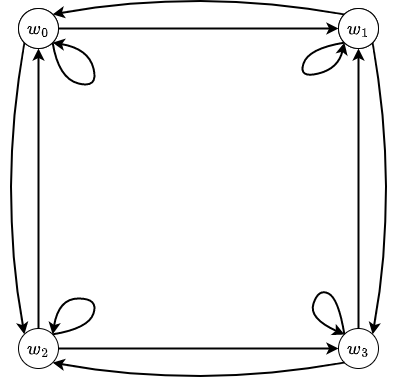
\includegraphics[width=0.5\linewidth]{ToUse/Paper discards/Images/2x2-cyclical-min-trans-equivalence.png}
    \caption{Transition equivalence classes in $D/\sim$ for the transitions shown in Figure \ref{fig:2x2-cyclical-min-trans}.}
    \label{fig:2x2-cyclical-min-trans-equivalence}
\end{figure}

\whendraft{
\textbf{FOR ABOVE FIGURE - equivalent transitions - include equivalence classes for minimum transitions.}
}

%%%%%%%%%%%%%%%%%%%%%%%%%%%%%%%%%%%%%%%%%%%%%%%
\subsection{Reversible transitions.}

Now we have an equivalence of transitions, we can define how a particular transition can be reversed by another transition.
This is a step towards defining the reversibility of actions, which is necessary for the action algebras to have the inverse property of groups.


\textbf{Reversible with respect to $\sim$.}
We call a transition $d \in D$ \textit{reversible} with respect to $\sim$, if there exists a transition $d' \in D$ that satisfies  $d \circ d' \sim 1_{s(d)}$ and $d' \circ d \sim 1_{s(d')}$.
Due to the definition of equivalence $\sim$, this means that $s(d)=t(d')$ and $t(d)=s(d')$.
A transition that is not reversible is called \textit{irreversible}.

If such a $d'$ exists, then we call $d'$ an \textit{inverse} of $d$ with respect to $D$.
When $D$ is clear from the context we simply say that $d$ is reversible.
We call the set of reversible transitions $D_{R}$.
\whendraft{\textbf{THOUGHT:} redefine reversible with respect to $\sim$ as $a' \circ a \sim 1$?}

\begin{figure}
    \centering
    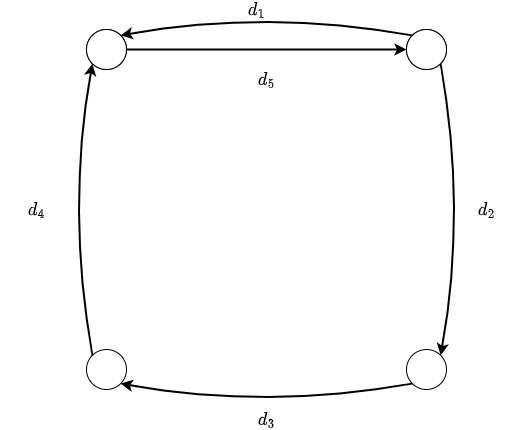
\includegraphics[width=0.5\linewidth]{ToUse/Paper discards/Images/reversible-composition.png}
    \caption{    
    Transition diagram of a reversible transition.
    Only minimum transitions $d_{1}$, $d_{2}$, $d_{3}$ and $d_{4}$ are minimum transitions.
    The only non-minimum transition shown is $d_{5} = d_{4} \circ d_{3} \circ d_{2} \circ d_{1}$; others are omitted for clarity.
    The transitions $d_{5}$ and $d_{1}$ are inverses of each other.
    }
    \label{fig:reversible-composition}
\end{figure}

Consider the transitions shown in Figure \ref{fig:reversible-composition}, where $d_{5} = d_{4} \circ d_{3} \circ d_{2} \circ d_{1}$.
The transition $d_{1}$ is reversible because there is the transition $d_{5}$ that satisfies $d_{5}: t(d_{1}) \xrightarrow{} s(t_{1})$; this means that $d_{5}$ is an inverse of $d_{1}$.
In fact, all the transitions shown are reversible since there is always a way to return to the source of any transition after the transition takes place by following the cycle given by transitions $d_{1}$, $d_{2}$, $d_{3}$, and $d_{4}$.

\begin{proposition}
    Any trivial transitions $1_{w} \in D$ is reversible and, for any trivial transition $1_{w}$, $1_{w}$ is an inverse of $1_{w}$.
\end{proposition}\begin{proof}
    Any trivial transition $1_{w} \in D$ has $s(1_{w})=t(1_{w})$ by definition.
    Therefore, the same trivial transition $1_{w}$ satisfies the conditions for being an inverse of $1_{w}$.
\end{proof}

\begin{proposition}
    If $d$ is reversible, then all elements of $[d]_{\sim}$ are reversible.
\end{proposition}
\begin{proof}
    [To do.]
\end{proof}

\begin{proposition}
    All the inverses of the elements of $d$ form an equivalence class.
\end{proposition}
\begin{proof}
    [To do.]
\end{proof}

\begin{proposition}
    If a transition $d \in D$ is reversible and $d'$ is an inverse of $d$, then $d'$ is also reversible with respect to $D$ and $d$ is an inverse of $d'$.
    
    \whendraft{
    \textbf{ILLUSTRATE in a sentence using transitions from running example}
    }
\end{proposition}\begin{proof}
    If $d \in D$ is reversible and $d' \in D$ is an inverse of $d$, then $s(d)=t(d')$ and $t(d)=s(d')$.
    This is also the condition for $d' \in D$ being reversible with respect to $D$ and $d'$ having $d$ as an inverse.
\end{proof}

\begin{proposition}\label{prp:composed-reversible-transitions-are-reversible}
    If two reversible transitions $d_{1},d_{2} \in D$, with inverses $d'_{1},d'_{2} \in D$ respectively, can be composed as $d_{2} \circ d_{1}$ then $d_{2} \circ d_{1}$ is also a reversible transition with $d'_{1} \circ d'_{2}$ as an inverse.
\end{proposition}
\begin{proof}
    If $d_{1}, d_{2}$ can be composed as $d_{2} \circ d_{1}$ then $t(d_{1})=s(d_{2})$.
    $s(d_{2} \circ d_{1})=s(d_{1})$ and $t(d_{2} \circ d_{1})=t(d_{2})$.
    By definition of an inverse of $d_{1}$, $d'_{1}$ has $s(d'_{1})=t(d_{1})$ and $t(d'_{1})=s(d_{1})$.
    Similarly, $d'_{2}$ has $s(d'_{2})=t(d_{2})$ and $t(d'_{2})=s(d_{2})$.
    Since $t(d'_{2})=s(d_{2})=t(d_{1})=s(d'_{1})$, $d'_{1}$ and $d'_{2}$ are composable as $d'_{1} \circ d'_{2}$, and $d'_{1} \circ d'_{2} \in D$.
    $s(d'_{1} \circ d'_{2})=s(d'_{2})=t(d_{2})$ and $t(d'_{1} \circ d'_{2})=t(d'_{1})=s(d_{1})$, which are the conditions for $d'_{1} \circ d'_{2}$ to be an inverse of $d_{2} \circ d_{1}$, and so $d_{2} \circ d_{1}$ is reversible.
\end{proof}

%%%%%%%%%%%%%%%%%%%%%%%%%%%%%%%%%%%%%%%%%%
\subsection{Equivalence of actions}

There exists a well-defined map $l_{\sim}$ such that the following diagram commutes:
\begin{figure}[H]
    \[\begin{tikzcd}
    {D_{A}} &&& A \\
    \\
    {D_{A}/\sim} &&& {A/\sim}
    \arrow["l", from=1-1, to=1-4]
    \arrow["{\pi_{D}}"', from=1-1, to=3-1]
    \arrow["{\pi_{A}}", from=1-4, to=3-4]
    \arrow["{l_{\sim}}"', from=3-1, to=3-4]
\end{tikzcd}\]

    \caption{Commutative diagram defining $l_{\sim}$.}
    \label{fig:Commutative_diagram_l}
\end{figure}

\begin{remark}
    \whendraft{
    \textbf{[This remark is not true - see notes in PhD Notebook 1.]}
    } 
    If $d \sim d'$, then $l(d) \sim l(d')$ for all $d, d' \in D_{A}$.
    This property ensures that $l_{\sim}$ is well-defined
    Therefore, if $d \in D_{A}$, with $l(d)=a$, maps to $[d] \in D_{A}/\sim$, $l_{\sim}([d])=[a]$.
\end{remark}

\paragraph{Reversible actions.}
Let $D_{AR}$ be the set of reversible transitions in $D_{A}$ ($D_{AR}=D_{A} \cap D_{R}$).
Consider a world state $w \in W$.
The set of reversible actions with $w$ is denoted $A_{Rw}$: $A_{R w} = \{a \in A \mid d: w \xrightarrow{a} t(d) \text{ and } d \in D_{AR} \}$.
An action $a \in A$ is called \textit{reversible} in a given state $w \in W$ if $a \in A_{R w}$.
If $A_{Rw} = A_{Rw'}$ for all $w, w' \in W$, then we denote all the $A_{Rw}$ as $A_{R}$.

\textbf{[Keep this ?]}
The properties of $A$, and therefore of $A/\sim$, are determined by the structure of the set of transitions $D_{A}$.
If a property involving $(A/\sim, \circ, *)$ or $(A, \circ, *)$ holds from any initial world state, then we can say it is a property of $(A/\sim, \circ)$ or $(A, \circ)$ respectively.


\textbf{
[Removed because these world conditions are no longer relevant.]
}



%%%%%%%%%%%%%%%%%%%%%%%%%%%%%%%%%%%%%%%%%%%%%%%%%%%%%%%%%%%%%%%%%%%%%%%%%%%%%%%%%%%%%%%%
\subsection{Conditions for SBDRL to apply}

\begin{world_condition}[If an action is reversible from one world state then it is reversible in all world states]\label{wldcon:action-always-reversible}
    For any action $a \in A$, if there exists a transition $d \in D_{AR}$ with $d: s(d) \xrightarrow{a} t(d)$ then all transitions in $d' \in D_{A}$ with $d': s(d') \xrightarrow{a} t(d')$ are also in $D_{AR}$.

\whendraft{
    Mathematically: If $a' \circ a * w_{i} = w_{i}$, then for any $w_{j} \in W$ there exists an $a'' \in A$ such that $a'' \circ a * w_{j} = w_{j}$.
}
\end{world_condition}

\begin{world_condition}[All transitions are reversible]\label{wldcon:all-transitions-reversible}
    $D=D_{R}$.
    This implies that $A=A_{R}$.
    \whendraft{
    \textbf{IS THIS TRUE ?}
    }

    \whendraft{\textit{Mathematically:} If $a * w_{i} = w_{j}$ then there exists $a' \in A$ such that $a' * w_{j} = w_{i}$ and therefore $a' \circ a * w_{i} = w_{i}$.
    }
\end{world_condition}

\begin{proposition}
    \hyperref[wldcon:action-homogeneity]{World condition \ref*{wldcon:action-homogeneity}} implies \hyperref[wldcon:action-always-reversible]{world condition \ref*{wldcon:action-always-reversible}}.
\end{proposition}
\begin{proof}
    Consider an action $a \in A$ that is reversible from a world state $w \in W$.
    From the definition of reversible actions, there must exist an $a' \in A$ such that $(a' \circ a) * w = w$.
    If \hyperref[wldcon:action-homogeneity]{world condition \ref*{wldcon:action-homogeneity}} is satisfied, it follows that for any world state $w' \in W$ $(a' \circ a) * w' = w'$, and so $a'$ is an inverse of $a$ from the world state $w'$.

    \whendraft{
    \textbf{ALTERNATIVE:}
    Consider an action $a \in A$ that is reversible from a world state $w \in W$; there exists a transition $d: w \xrightarrow{a} t(d)$.
    From the definition of reversible actions, there exists a transition $d': t(d) \xrightarrow{a'} w$.
    If \hyperref[wldcon:action-homogeneity]{world condition \ref*{wldcon:action-homogeneity}} is satisfied, then for any $w' \in W$ there must exist a transition $d'': \sigma(w, w')(w) \xrightarrow{a} \sigma(w, w')(t(d)$ and a transition $d''': \sigma(w, w')(t(d) \xrightarrow{a'} \sigma(w, w')(w)$.
    Therefore $(a' \circ a) * w' = w'$, and so $a'$ is an inverse of $a$ from the world state $w'$.
    }
\end{proof}


\begin{proposition}
    If a world satisfies \hyperref[wldcon:action-homogeneity]{world condition \ref*{wldcon:action-homogeneity}} and an action $a \in A$ is defined in at least one world state then it is defined in all world states.
    It immediately follows that if a world satisfies \hyperref[wldcon:action-homogeneity]{world condition \ref*{wldcon:action-homogeneity}} and every action $a \in A$ is defined in at least one world state, then \hyperref[wldcon:unrestricted-actions]{world condition \ref*{wldcon:unrestricted-actions}} is satisfied.
\end{proposition}
\begin{proof}
    If $a * w$ is defined for a world state $w \in W$, then there exists a world state $w'$ such that $a * w = w'$.
    If \hyperref[wldcon:action-homogeneity]{world condition \ref*{wldcon:action-homogeneity}} is satisfied, then for any $w'' \in W$ there must exist a world state $w''' \in W$ such that $a * w'' = w'''$, and so $a * w''$ is defined.
    Since the choice of $w''$ is arbitrary, then \hyperref[wldcon:unrestricted-actions]{world condition \ref*{wldcon:unrestricted-actions}} is satisfied.

    \whendraft{
    \textbf{ALTERNATIVE:}
    If $a * w$ is defined for a world state $w \in W$, then there exists a transition $d: w \xrightarrow{a} t(d)$.
    If \hyperref[wldcon:action-homogeneity]{world condition \ref*{wldcon:action-homogeneity}} is satisfied, then for any $w' \in W$ there must exist a transition $d': \sigma(w, w')(w) \xrightarrow{a} \sigma(w, w')(t(d)$, and so $a * w'$ is defined.
    Since the choice of $w'$ is arbitrary, then \hyperref[wldcon:unrestricted-actions]{world condition \ref*{wldcon:unrestricted-actions}} is satisfied.
    }
\end{proof}


%%%%%%%%%%%%%%%%%%%%%%%%%%%%%%%%%%%%%%%%%%%%%%%
\subsection{Sufficient conditions}

In this section, we show that the transformations of a world obeying world conditions \ref{wldcon:action-always-reversible}, \ref{wldcon:all-transitions-reversible}, \ref{wldcon:unrestricted-actions}, and \ref{wldcon:action-homogeneity} can be fully described by a group action, and therefore can be fully described by the formalism given by \cite{Higgins2018}.

\begin{proposition}\label{prp:Asim-closed-1-5}
    We show here that the elements of $A/\sim$ are defined for every world state if the world obeys world condition \ref{wldcon:unrestricted-actions}.
\end{proposition}
\begin{proof}
    Consider any two actions $a_{1}, a_{2} \in A$, and consider a transition $d_{1}: s(d_{1}) \xrightarrow{a_{1}} t(d_{1})$.
    There exists a transition $d_{2}: t(d_{1}) \xrightarrow{a_{2}} t(d_{2})$ because actions are unrestricted in $W$.
    $\implies$ there exists a transition $(d_{2} \circ d_{1}): s(d_{1}) \xrightarrow{a_{2} \circ a_{1}} t(d_{2})$, and therefore $(a_{2} \circ a_{1}) \in A$.
    Therefore, $(A/\sim, \circ)$ is closed.
\end{proof}

\begin{proposition}\label{prp:Asim-inverse-1-5}
    If the world obeys world conditions \ref{wldcon:action-always-reversible}, \ref{wldcon:all-transitions-reversible}, \ref{wldcon:unrestricted-actions} and \ref{wldcon:action-homogeneity}, then every element in $(A/\sim, \circ)$ has an inverse element .
\end{proposition}
\begin{proof}
    To show that every element in $(A/\sim, \circ)$ has an inverse element, we must show that for every $a \in A$, there exists $a' \in A$ such that (a) $[a']_{\sim} \circ [a]_{\sim} = [1]_{\sim}$ and (b) $[a]_{\sim} \circ [a']_{\sim} = [1]_{\sim}$.
    
    Consider any transition $d_{1}: s(d_{1}) \xrightarrow{a} t(d_{1})$, which is labelled by any action $a \in A$.
    $a$ is reversible $\implies$ $d_{1}$ is reversible $\implies$ there exists transition $d'_{1}: t(d_{1}) \to s(d_{1})$.
    Since $a$ is reversible, $d'_{1} \in D_{A}$ (by definition of reversible action).
    Let us denote the label of $d'_{1}$ by $a'$ so $d'_{1}: t(d_{1}) \xrightarrow{a'} s(d_{1})$.
    
    (a) $t(d_{1}) = s(d'_{1})$ $\implies$ there exists $(d'_{1} \circ d_{1}): s(d_{1}) \xrightarrow{a' \circ a} s(d_{1})$.
    $s(d'_{1} \circ d_{1})=t(d'_{1} \circ d_{1})$ $\implies$ $a' \circ a \sim 1$.
    $\implies$ $[a' \circ a]_{\sim} = [1]_{\sim}$.
    $\implies$ $[a']_{\sim} \circ [a]_{\sim} = [1]_{\sim}$.
    
    (b) Since $W$ is action homogeneous, we can use the existence of the action homogeneity bijection $\sigma_{(t(d_{1}), s(d_{1}))}$, which sends $t(d_{1}) \mapsto s(d_{1})$, to deduce that the following transitions must exist: $d_{2}: s(d_{2}) \xrightarrow{a} s(d_{1})$ and $d'_{2}: s(d_{1}) \xrightarrow{a'} s(d_{2})$, where $s(d_{2}) = \sigma_{(t(d_{1}), s(d_{1}))}(s(d_{1}))$.
    $t(d'_{2}) = s(d_{2})$ $\implies$ there exists $(d_{2} \circ d'_{2}): s(d_{1}) \xrightarrow{a \circ a'} s(d_{1})$.
    $s(d_{2} \circ d'_{2}) = t(d_{2} \circ d'_{2})$ $\implies$ $a \circ a' \sim 1$.
    $\implies$ $[a \circ a']_{\sim} = [1]_{\sim}$.
    $\implies$ $[a]_{\sim} \circ [a']_{\sim} = [1]_{\sim}$.
\end{proof}

\begin{proposition}\label{prp:Asim-group-1-5}
    If the world obeys world conditions \ref{wldcon:action-always-reversible}, \ref{wldcon:all-transitions-reversible}, and \ref{wldcon:action-homogeneity} then $(A/\sim, \circ)$ is a group.
\end{proposition}
\begin{proof}
    Closure is given by \hyperref[prp:Asim-closed-1-5]{proposition \ref*{prp:Asim-closed-1-5}}.
    Associativity is given by \hyperref[prp:Asim-associative-1-5]{proposition \ref*{prp:Asim-associative-1-5}}.
    Identity element given by \hyperref[prp:Asim-identity-1-5]{proposition \ref*{prp:Asim-identity-1-5}}.
    Inverse element given by \hyperref[prp:Asim-inverse-1-5]{proposition \ref*{prp:Asim-inverse-1-5}}.
\end{proof}

\begin{remark}
    Since $(A/\sim, \circ)$ is a group, we automatically know more features of $(A/\sim, \circ)$ such as $[1]_{\sim}$ is the only action that satisfies the condition to be an identity element of $(A/\sim, \circ)$, and that each element of $(A/\sim, \circ)$ has exactly one inverse element in $(A/\sim, \circ)$.
\end{remark}

We have considered some of the properties of $(A/\sim, \circ)$ separately from $(A/\sim, \circ, *)$.
However, when considering $(A/\sim, \circ, *)$ itself, we see it forms a group action.

\begin{proposition}\label{prp:action-homogeneity-sufficient}
    If the world obeys world conditions \ref{wldcon:action-always-reversible}, \ref{wldcon:all-transitions-reversible}, and \ref{wldcon:action-homogeneity}, then $\psi: (A/\sim) \times W \to W$, where $\psi([a]_{\sim}, w) = [a]_{\sim} * w$, is a left group action.
\end{proposition}
\begin{proof}
    We have already established that $(A/\sim, \circ)$ is a group (see \hyperref[prp:Asim-group-1-5]{proposition \ref*{prp:Asim-group-1-5}}.
    Therefore, to show that $\psi$ is a left group action we only have to prove the group action conditions of (a) identity and (b) compatibility.
    Consider an arbitrary world state $w_{1} \in W$.
    
    (a) $\psi([1]_{\sim}, w_{1}) = [1]_{\sim} * w_{1} = 1 * w_{1} = 1_{w_{1}} * w_{1} = w_{1}$.
    
    (b) Need to show that $\psi(a', \psi(a, w_{1})) = \psi(a' \circ a, w_{1})$.
    Because actions are unrestricted in $W$, for any $w_{1} \in W$, there exists the transitions $d_{1}: w_{1} \xrightarrow{a} t(d_{1})$ and $d_{2}: t(d_{1}) \xrightarrow{a} t(d_{2})$.
    $\implies$ there exists the transition $(d_{2} \circ d_{1}): w_{1} \xrightarrow{a' \circ a} t(d_{2})$.
    Therefore, $\psi(a' \circ a, w_{1}) = (a' \circ a) * w_{1} = t(d_{2})$.
    Using the transitions $d_{1}, d_{2}$ for the LHS of the condition, $\psi(a', \psi(a, w_{1})) = \psi(a', a * w_{1}) = \psi(a', t(d_{1})) = a' * t(d_{1}) = t(d_{2})$.
\end{proof}

%%%%%%%%%%%%%%%%%%%%%%%%%%%%%%%%%%%%%%%%%%%%%%%
\subsection{Necessary conditions}

In this section, we show that world conditions \ref{wldcon:action-always-reversible}, \ref{wldcon:all-transitions-reversible}, \textbf{4} and \ref{wldcon:action-homogeneity} are necessary conditions for fully describing the dynamics of a world by a group action, and therefore fully describing the dynamics of a world by the formalism given by \cite{Higgins2018}.
These conditions being necessary identifies limits of \cite{Higgins2018}'s formalism.

It is clear from the definition of a group that $(A/\sim) \times W \to W$ is not a group action in worlds that (1) do not have action reversibility (\hyperref[wldcon:all-transitions-reversible]{world condition \ref*{wldcon:all-transitions-reversible}}) because the inverse property is not satisfied, (2) worlds that do not have unrestricted actions (\textbf{world condition 4}) because the totality property is not satisfied, and (3) worlds that do not have action reversibility (world condition 2) because the inverse property is not satisfied.


\begin{proposition}\label{prp:action-homogeneity-necessary}
    If $(A/\sim) \times W \to W$ is a group action, then \hyperref[wldcon:action-homogeneity]{world condition \ref*{wldcon:action-homogeneity}} is satisfied.
\end{proposition}
\begin{proof}
    Consider a world whose labelled transformations satisfy SBDRL, but the world does not satisfy action homogeneity (\textbf{world condition 5}).
    Since the world's transformations satisfy SBDRL, the transformations of the world form a group action $(A/\sim) \times W \to W$.
    \textbf{Consider a world $(W, D_{A})$ without the action homogeneity condition, but with world conditions 1-4.}
    If there is no action homogeneity, then there exists at least one ordered pair $(w_{1}, w_{2})$ of world states, where $w_{1}, w_{2} \in W$, such that for any map $\sigma: W \to W$ with $\sigma(w_{1})=w_{2}$, there must be at least one transition $d:s(d) \xrightarrow{a} t(d)$ ($d \in D_{A}$, $a \in A$) for which there does not exist a transition $d_{\sigma}:\sigma(s(d)) \xrightarrow{a} \sigma(t(d))$.
    
    Now consider the world state $\sigma(t(d))$.
    By unrestricted actions (\hyperref[wldcon:unrestricted-actions]{world condition \ref*{wldcon:unrestricted-actions}}), there exists a transition $d_{2}: \sigma(t(d)) \xrightarrow{a} t(d_{2})$.
    Therefore, by reversible actions (\hyperref[wldcon:action-always-reversible]{world condition \ref*{wldcon:action-always-reversible}} and \hyperref[wldcon:all-transitions-reversible]{world condition \ref*{wldcon:all-transitions-reversible}}), there must be a transition $d'_{2}: t(d_{2}) \xrightarrow{a'} \sigma(t(d))$ such that, by the definition of group action, $a' \circ a \sim 1$.
    By unrestricted actions, there must be a transition $d'_{3}: \sigma(t(d)) \xrightarrow{a'} t(d'_{3})$.
    Therefore, by reversible actions, there must exist a transition $d_{3}: t(d'_{3}) \xrightarrow{a_{2}} \sigma(t(d))$ such that, by the definition of group action, $a_{2} \circ a' \sim 1$.
    
    There are now two possibilities:
    \begin{enumerate}
        \item $a_{2} \neq a$, and so the left inverse of $[a']_{\sim}$ is different to the right inverse of $[a']_{\sim}$; one of the properties of a group is that the inverse of a group element is unique and so the right and left inverses of a group element must be the same. This is not the case here and therefore would mean that $(A/\sim, \circ)$ is not a group and so $(A/\sim) \times W \to W$ is not a group action.
        
        \item $a_{2} = a$, and so $d_{3}$ is a transition with $d_{3}: \sigma(s(d)) \xrightarrow{a} \sigma(t(d))$, which is a contradiction because it has already been shown that such a transition cannot exists if the world does not have the action homogeneity property.
    \end{enumerate}


    
    Therefore, without $W$ satisfying the action homogeneity condition, $(A/\sim) \times W \to W$ is not a group action.
\end{proof}

Therefore, to be able to describe the dynamics of a world using SBDRL a world must satisfy \hyperref[wldcon:agent-actions-only]{world condition \ref*{wldcon:agent-actions-only}}, \hyperref[wldcon:all-transitions-reversible]{world condition \ref*{wldcon:all-transitions-reversible}}, \textbf{world condition 4}, and \hyperref[wldcon:action-homogeneity]{world condition \ref*{wldcon:action-homogeneity}}.

%%%%%%%%%%%%%%%%%%%%%%%%%%%%%%%%%%%%%%%%
\subsection{Notes}

\subsection{Reminder of Higgins}

Observation process: $b: W \to O$.
Inference process: $h: O \to Z$.
Composite mapping: $f = h \circ b: W \to Z$.

The set $W$ of world states has a set of symmetries that are described by the group $G$, which acts on the set of world states via a group action $\cdot_{W}: G \times W \to W$ that sends $(g, w_{1}) \mapsto g \cdot_{W} w_{1} = w_{2}$.
For the agent's representations $z_i \in Z$ to be symmetry-based representations, a corresponding group action $\cdot_{Z}: G \times Z \to Z$ that sends $(g, z_1) \mapsto z_2 \ \forall g \in G, \ \forall z_i \in Z$, where $f(w_1) = z_1$ and $f(w_2) = z_2$, must be found so that the symmetries of the agent's representations reflect the symmetries of the world states.
the mathematical condition for symmetry-based representations with respect to the group $G$ is $f(g \cdot_W w_1) = g \cdot_Z f(w_1)$.

\subsection{What do we want?}

We want to answer the following questions:
\begin{enumerate}
    \item In which worlds does the set $A$ of all the transitions in the world form a group?
    
    \item In which worlds does the action $A \times W$ form a group action?
\end{enumerate}

\textbf{Other questions:}
\begin{enumerate}
    \item Are there worlds where $A$ is not a group, but there exists a subset $G \subset A$ which is a group and does form a group action $G \times W \to W$?
    
    \item Do the minimum actions need to be the generators of the group?
    \begin{itemize}
        \item No - e.g., if one or more minimum actions generate another minimum action.
    \end{itemize}
\end{enumerate}

\subsection{Relevant concepts}

\textbf{Group action.}
Let $G$ be a group and let $X$ be a set.
A (left) group action $*: G \times X \to X$, $(g,x) \mapsto g * x$ is a function from the Cartesian product that is compatible with the group's structure: for all $x \in X$ and for all $g,h \in G$, $e * x = x$, where $e$ is the identity element of $G$, and $g * (h * a) = (g h) * a$.

\textbf{Cayley graph.}
Let $G$ be a group and let $S \subseteq G$ be a set of group elements such that the identity element $e \not\in S$.
The Cayley graph associated with $(G, S)$ is defined as the directed graph having one vertex associated with each group element and directed edges $(g,h)$ whenever $g h^{-1} \in S$.
The Cayley graph may depend on the choice of a generating set.
The Cayley graph is connected iff $S$ generates $G$.
A direct graph Cayley graph has the same edge multiplicity for each vertex (i.e., every vertex has the same number of edges sharing that end vertex).
A Cayley graph is always vertex-transitive, but not all vertex-transitive graphs are Cayley graphs.

\textbf{Groups and graphs.}

\subsection{Conditions for $A \times W$ group action}

\begin{itemize}
    \item Is the condition just that (some set of?) the minimum actions have to generate a group or can we find a more restrictive condition?
    
    \item Not just the conditions for the actions to form a Cayley graph with the world states as vertices ?
\end{itemize}


%%%%%%%%%%%%%%%%%%%%%%%%%%%%%%%%%%%%55
\section{Beyond SBDRL}

\begin{definition}[Monoid]
    A `monoid' is a set $S$ equipped with a binary operation $\circ: S \times S \to S$ that satisfies the following axioms:
    \begin{enumerate}
        \item For all $a,b,c, \in S$, the equation $(a \circ b) \circ c = a \circ (b \circ c)$ holds.
        \item There exists an element $e \in S$ such that for every element $e \in S$, the equations $e \circ a = a$ and $a \circ e = a$ hold.
    \end{enumerate}
\end{definition}


\subsection{A more granular equivalence of actions.}

\begin{itemize}
    \item Is the map $l$ well defined for action homogeneous worlds only ? - if so, then the following would be true for action-homogeneous worlds: ``Consider $d_{1}: s(d_{1}) \xrightarrow{a} t(d_{1})$ and $d_{2}: s(d_{1}) \xrightarrow{a'} t(d_{1})$, so $d_{1} \sim d_{2}$.
    Using the previously given definition of $\sim$ on $A$, this implies that $a \sim a'$.''
\end{itemize}

Consider $d_{1}: s(d_{1}) \xrightarrow{a} t(d_{1})$ and $d_{2}: s(d_{1}) \xrightarrow{a'} t(d_{1})$, so $d_{1} \sim d_{2}$.
Using the previously given definition of $\sim$ on $A$, this implies that $a \sim a'$ \textbf{(This is wrong - can have separate notions of weak equivalence for transitions and actions though. Problem with Hugo's commutative action sequences paper?)}.
However, in worlds without action-homogeneity (\textit{i.e.}, action-inhomogeneous worlds), it is possible to also have $d_{3}: s(d_{3}) \xrightarrow{a} t(d_{3})$ and $d_{4}: s(d_{3}) \xrightarrow{a'} t(d_{3})$, and so $d_{3} \not\sim d_{4}$.
Once again using the previously given definition of $\sim$ on $A$, this implies that $a \not\sim a'$.

This section only considers worlds where all transitions are due to the actions of an agent and all actions are reversible (when considering the actions from a specified starting state).
First, we will consider worlds where actions are sometimes restricted.
For example, consider an agent that can move left, right, up, and down in a 2D Euclidean world; if the world is cyclical (\textit{i.e.}, continuing to move in one direction will eventually cause the agent to return to its original position), then the world is action-homogeneous; however, if we place a wall, which prevents movement, to the right of the agent, then the agent's `move to the right' action is restricted when the agent is in the position directly to the left of the wall; this makes the world action-inhomogeneous and breaks the symmetry of the agent's actions so they cannot be described as a group action on the set of world states.

To explore the contradiction in the previous definition of $\sim$, we consider the transitions starting from a particular world state $w \in W$ and the actions $a \in A$ of an agent associated with those transitions.

\begin{definition}[$D_{w}$]
    Let $D_{A w}$ be the set of all transitions due to the actions of an agent with source $w$ and the inverses, where they exist, of these actions.
    
    $D_{A w} := \{d \mid d \in D_{A}\textit{ such that } s(d)=w\textit{ or }t(d)=w\}$
\end{definition}

\begin{definition}
    $A_{w} := \{a \mid a=l(d), d \in D_{A w}\}$
\end{definition}

We now adapt our relation $\sim$ to the transitions $D_{w}$.

\begin{definition}[$\sim_{w}$]
    $d_{1} \sim_{w} d_{2}$ if $d_{1},d_{2} \in D_{A w}$ and $t(d_{1})=t(d_{2})$.
\end{definition}

\begin{remark}
    This definition is the same as the definition of $\sim$, but considering a subset of the transitions in $D$ only.
\end{remark}

\begin{definition}[$\sim_{w}$]\label{def:action equivalence w}
    For $a,a' \in A$ and $w \in W$, $a \sim_{w} a$ if $a * w = a' * w$ or $a$ and $a'$ are both restricted actions with respect to $w$.
\end{definition}

\begin{remark}
    In definition \ref{def:action equivalence w}, for the case where $a,a'$ are both restricted actions, then we say $a * w = a' * w$.
    The meaning of $a * w$ where $a$ is restricted on $w$ will be defined later.
\end{remark}

        % #TODO: include parts about restricted actions.
\begin{proposition}
    $\sim_{w}$ is an equivalence relation.
\end{proposition}
\begin{proof}
    To show that $\sim_{w}$ is an equivalence relation, we need to show that the relation is (a) reflexive, (b) transitive, and (c) symmetric.
    (a) For a binary relation $R$ over a set $X$ to be reflexive: $x R x$ for every $x \in X$. For $w \in W$, if $\exists a * w$ then $a * w = a * w$ from the properties of $=$ for any $a \in A$. Therefore, $a \sim_{w} a$.
    (b) For a binary relation $R$ over a set $X$ to be transitive: if $a R b$ and $b R c$ then $a R c$ for all $a,b,c \in X$.
    If $a \sim_{w} a'$ and $a' \sim_{w} a''$, then $\exists a * w$, $\exists a' * w$, $\exists a'' * w$, and $a * w = a' * w$, $a' * w = a'' * w$ for all $w \in W' \subseteq W$.
    The two equations can be used to show that $a * w = a'' * w$.
    This, along with the already established $\exists a * w$ and $\exists a'' * w$, is the condition for $a \sim_{W'} a''$.
    (c) For a binary relation $R$ over a set $X$ to be reflexive: if $a R b$, then $b R a$ for all $a,b \in X$.
    If $a \sim_{W'} a'$, then $\exists a * w$, $\exists a' * w$, and $a * w = a' * w$. Therefore $a' * w = a * w$.
    This, along with the already established $\exists a * w$ and $\exists a' * w$, is the condition for $a' \sim_{W'} a$.
\end{proof}

We now consider two prominent methods for dealing with restricted actions in AI literature: masking restricted actions, and treating restricted actions as identity actions, and then consider worlds that are action inhomogeneous but do not contain restricted actions.


\subsection{Treating restricted actions as identity actions}\label{sec:Treating restricted actions as identity actions}
\whendraft{
\noindent\rule{\textwidth}{1mm}
\begin{itemize}
    \item If restricted actions are treated as being in the same equivalence class as the trivial action, then:
    \begin{itemize}
        \item the uniqueness of inverse fails (?) but totality is maintained and so $A_{w}/\sim_{w}$ is an inverse semigroup ?
        \begin{itemize}
            \item Each element has a right inverse and a left inverse, but right inverse is not necessarily the same as the left inverse.
        \end{itemize}
        \item $A_{w}/\sim_{w}$ is a group, but is a different group for different $w \in W$? - \textbf{Doesn't look like it.}
    \end{itemize}
    
    \item Show category groupoid ($A_{w}/\sim_{w})$.
    
    \item Strangely, $A_{w}$ on $\sim_{w}$ appears to be a monoid with left inverse always present ?
    \begin{itemize}
        \item But `Any Set with Associativity, Left Identity, Left Inverse is a Group' % https://math.stackexchange.com/questions/537572/any-set-with-associativity-left-identity-left-inverse-is-a-group
        \item It appears that each element of $A_{w}$ has a left inverse under $\sim_{w}$, but that left inverses do not necessarily decompose to minimum actions ?
    \end{itemize}
\end{itemize}
\noindent\rule{\textwidth}{1mm}
}

\whendraft{
\begin{figure}[H]
    \centering
    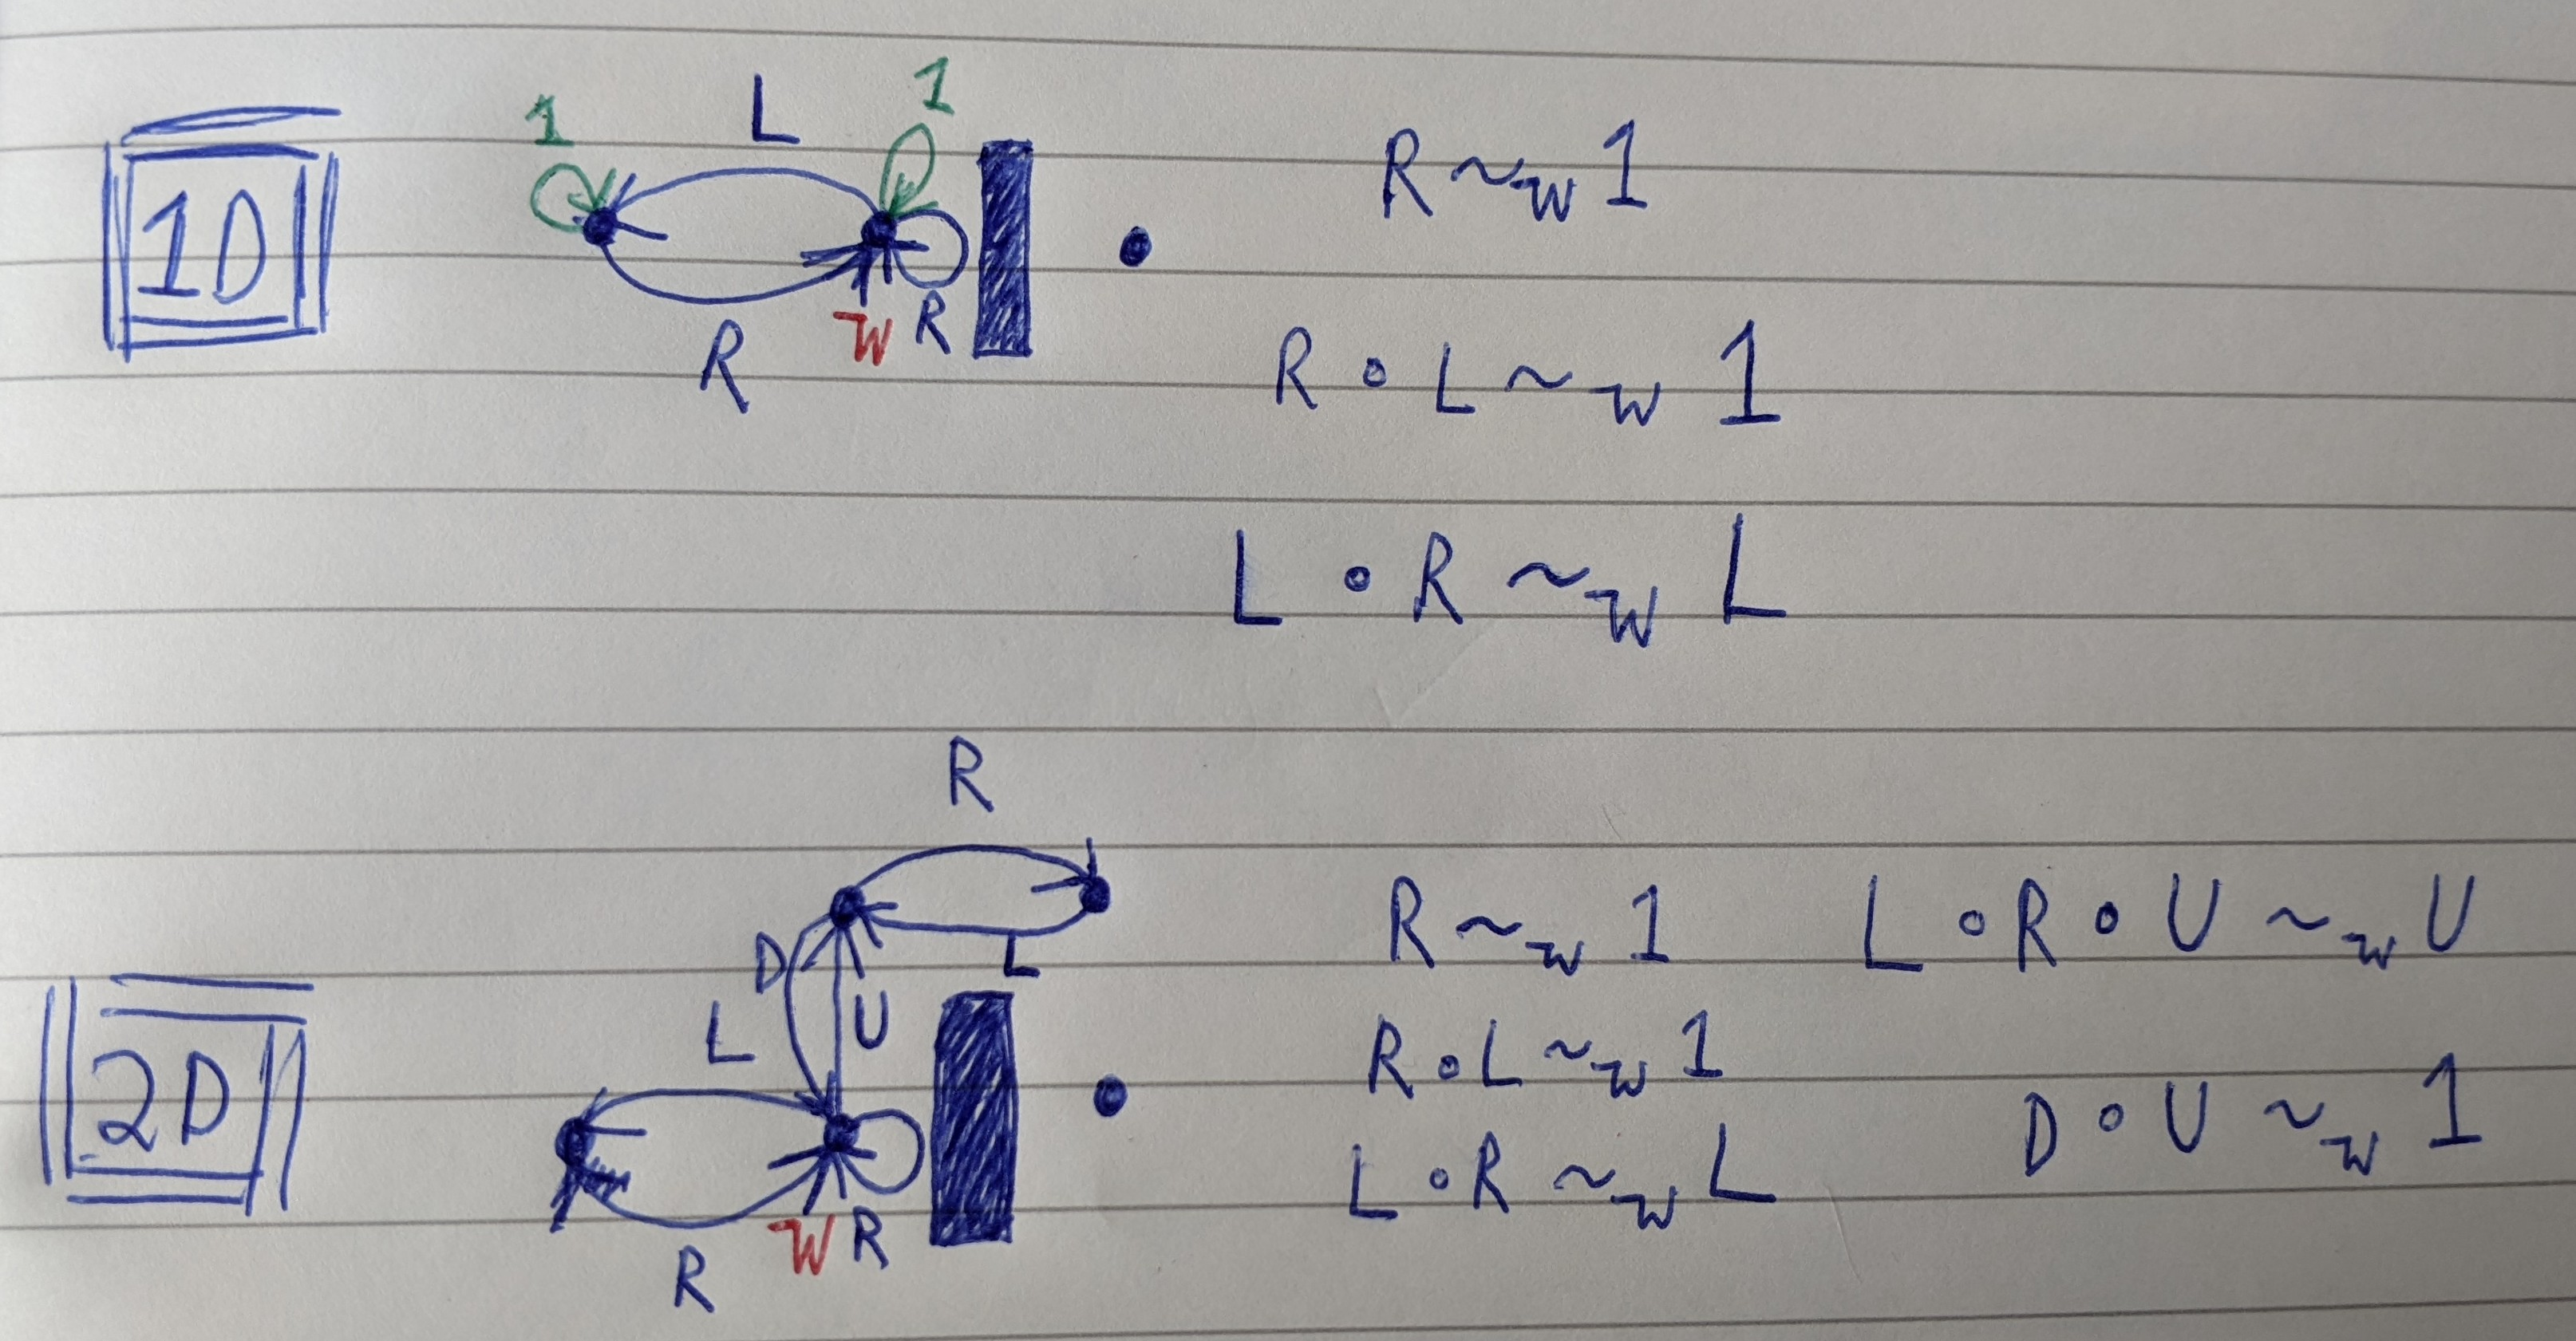
\includegraphics[width=\textwidth]{ToUse/Paper discards/Images/fig-restricted-as-identity-example.jpg}
    \caption{Example of sections of a 1D world with restricted actions and a 2D restricted world with restricted actions}
    \label{fig:restricted-as-identity-example}
\end{figure}
}


\whendraft{
An example of this is shown in Figure \ref{fig:restricted-as-identity-example}: in the 1D example, the left inverse of $L$ is $R$, but there appears to be no right inverse of $L$ (\textit{i.e.}, there is no $x \in A$ such that $L \circ x \sim_{w} 1$); in the 2D example, there now appears to be a right inverse of $L$, but only if $U$ is the first action performed from $w$ since $L \circ R \circ U \sim_{w} U$ and $U \sim_{w} U$.
}



\draftnote{blue}{awjdean}{
\textbf{How to deal with composition?}
$a\circ b$ where $a$ unrestricted, $b$ restricted.
$a\circ b$ where $a$ restricted, $b$ unrestricted.
$a\circ b$ where $a,b$ restricted.
$a\circ b$ where $a,b$ unrestricted, but $a \circ b$ restricted.
}

\draftnote{blue}{awjdean}{
\textbf{Properties that indicate dimensionality.}
Dimensionality indicator using 'planes' of commutativity.
}

\subsection{Irreversible homogeneous actions}\label{sec:Irreversible homogeneous actions}
\whendraft{
\noindent\rule{\textwidth}{1mm}
\textbf{Notes:}
\begin{enumerate}
    \item Examples of homogeneous irreversible actions:
    \begin{itemize}
        \item Suicide button.
        \item Colour change action with infinite spectrum of colours.
        \item Number generating button $\to$ generating digits of pi.
    \end{itemize}

    \item \textit{Hypothesis:} world with irreversible actions can only be action homogeneous until an irreversible action is performed?
    \begin{itemize}
        \item \textit{Possible counter example:} agent can perform irreversible action of `opening new (perpendicular) cyclical movement dimension' in any state (\textit{i.e.}, cyclical 2D $\to$ cyclical 3D world).
    \end{itemize}
    
    \item Structure of world is described by monoid action.
    \item \textit{Hypothesis:} Reversible actions and irreversible actions must commute and therefore form different subspaces in an agent's representation.
    
    \item \textbf{Conjecture.} In real world scenarios, performing a homogeneous irreversible action makes the world inhomogeneous $\to$ no, if infinite sequence (e.g., digits of pi).
    
    \item Resources:
        % http://settheory.net/algebra/monoid-actions#:~:text=An%20action%20(or%20left%20action,%E2%8B%85(b%E2%8B%85x).
        
        % https://en.wikipedia.org/wiki/Semiautomaton

\end{enumerate}
\noindent\rule{\textwidth}{1mm}
}

In this section, we explore the action algebras of worlds with transformations that form algebras that are action-homogeneous but contain irreversible actions.
We have chosen to consider worlds with action homogeneity and irreversible actions first because we hypothesised that their treatment would be similar to that of reversible worlds with action homogeneity.




\begin{proposition}
    For any action homogeneous world $W$ and any $w \in W$, $A_{w}/\sim_{w}$ is a monoid.
\end{proposition}
\begin{proof}    \textbf{Identity.} Present by action condition 1.
    \textbf{Associativity.} Present by associativity of $\circ$.
\end{proof}

\begin{proposition}
    For $w, w' \in W$, the monoid $A_{w}/\sim_{w}$ is isomorphic to the monoid $A_{w'}/\sim_{w'}$.
\end{proposition}
\begin{proof}
    True by action homogeneity.
    Previous proposition shows that $A_{w}/\sim_{w}$ is a monoid for any $w \in W$; now invoke the homomorphism of the action homogeneity condition to show these monoids are isomorphic with respect to their generators.
\end{proof}

\begin{remark}
    The dynamics of an action-homogeneous world that is only affected by the actions of an agent are fully described by the monoid action $(A_{w}/\sim_{w}) \times W \to W$, for any $w \in W$.
\end{remark}

\whendraft{
\begin{proof}
    
    \textbf{Proof for the above remark:}
    We have every $(A_{w}/\sim_{w}) \times w$ being isomorphic, therefore can group the $w$'s so that $(A_{w}/\sim_{w}) \times W \to W'$ where $W' \subseteq W$.
    Now show that $W' = W$: if $W' \neq W$, then $W$ must contain disjoint subsets.
\end{proof}
}

\whendraft{
\textbf{THOUGHT.}
Proposition: It's not possible to have a finite world with irreversible, homogeneous actions.
Consider if world has multiple homogeneous irreversible actions.
Consider if world has homogeneous irreversible actions that is reversible everywhere except one state (other (reversible) actions don't have to be action-homogeneous).
}





%%%%%%%%%%%%%%%%%%%%%%%%%%%%%%%%%%%%55
\section{Generalising SBDRL}

\subsection{World dynamics as categories}

Here we show that the transition algebras derived using the equivalence relation $\sim$ can be expressed as categories.

\paragraph{Transition multigraphs as categories.}

\begin{proposition}
    The elements in $D/\sim$ and the world states in $W$ form a category $\textbf{C}(Q_{D/\sim})$ with the elements of $D/\sim$ as morphisms and the elements of $W$ as objects.
\end{proposition}\begin{proof}
    To show that $\textbf{C}(Q_{D/\sim})$ is a category, we must show that the following conditions are satisfied: (a) composition of morphisms, (b) existence of units, and (c) associativity of composition of morphisms.
    
    (a) The morphisms are paths in the quiver $Q_{D/\sim}$, and composition of these paths is composition of morphisms in $\textbf{C}(Q_{D/\sim})$.
    If $[d]_{\sim}$ is a morphism in $\textbf{C}(w,w')$, then $[d]_{\sim}$ is a transition in $D/\sim$ with $s([d]_{\sim})=w$ and $t([d]_{\sim})=w'$.
    If $[d']_{\sim}$ is a morphism in $\textbf{C}(w',w'')$, then $[d']_{\sim}$ is a transition in $D/\sim$ with $s([d']_{\sim})=w'$ and $t([d']_{\sim})=w''$.
    Composition of paths means there is a transition $[d' \circ d]_{\sim}$ that is in $\textbf{C}(w, w'')$ because $[d' \circ d]_{\sim} \in D/\sim$, $s([d' \circ d]_{\sim})=s([d]_{\sim})=w$, and $t([d' \circ d]_{\sim})=t([d']_{\sim})=w''$.
    
    (b) For each world state $w$ in $W$, there is a trivial transition $[1_{w}]_{\sim} \in \textbf{C}(w,w)$, which is a transition in $D/\sim$ with $s([1_{w}]_{\sim})=w$ and $t([1_{w}]_{\sim})=w$.
    If $[d]_{\sim}$ is a morphism in $\textbf{C}(w,w')$, then $[d]_{\sim}$ is a transition in $D/\sim$ with $s([d]_{\sim})=w$ and $t([d]_{\sim})=w'$; therefore, due to composition of paths, $[d \circ 1_{w}]_{\sim} \in D/\sim$ with $s([d \circ 1_{w}]_{\sim})=s([1_{w}]_{\sim})=w$ and $t([d \circ 1_{w}]_{\sim})=s([d]_{\sim})=w'$; therefore, $[d \circ 1_{w}]_{\sim} = [d]_{\sim}$.
    Similarly, if $[d']_{\sim}$ is a morphism in $\textbf{C}(w'',w)$, then $[d']_{\sim}$ is a transition in $D/\sim$ with $s([d']_{\sim})=w''$ and $t([d]_{\sim})=w$; therefore, due to composition of paths, $[1_{w} \circ d']_{\sim} \in D/\sim$ with $s([1_{w'} \circ d']_{\sim})=s([d']_{\sim})=w''$ and $t([1_{w} \circ d']_{\sim})=t([1_{w}]_{\sim})=w$; therefore, $[1_{w} \circ d']_{\sim} = [d']_{\sim}$.
    
    (c) Composition of paths is associative, therefore the associativity condition of the composition of morphisms is satisfied.
\end{proof}

\begin{proposition}\label{prp:reversible-to-isomorphism}
    The equivalence classes with respect to $\sim$ of reversible transitions give isomorphisms in $\textbf{C}(Q_{D/\sim})$.
\end{proposition}\begin{proof}
    If $d: w \to w'$ is a reversible transitions in $D$ then there must be an inverse $d': w' \to w$ in $D$.
    $\pi_{\sim}$ sends $d' \circ d$ to $[d' \circ d]_{\sim}$ and $[d' \circ d]_{\sim} = [1_{w}]_{\sim}$.
    Similarly, $\pi_{\sim}$ sends $d \circ d'$ to $[d \circ d']_{\sim}$ and $[d \circ d']_{\sim} = [1_{w'}]_{\sim}$.
\end{proof}

\begin{proposition}
    $\textbf{C}(Q_{D_{R}/\sim})$ is a groupoid.
\end{proposition}\begin{proof}
    Every transition in $D_{R}$ is reversible by \hyperref[prp:composed-reversible-transitions-are-reversible]{proposition \ref*{prp:composed-reversible-transitions-are-reversible}}.
    Every reversible transition gives an isomorphism in $\textbf{C}(Q_{D_{R}/\sim})$ by \hyperref[prp:reversible-to-isomorphism]{proposition \ref*{prp:reversible-to-isomorphism}}.
    Therefore, $\textbf{C}(Q_{D_{R}/\sim})$ is a groupoid.
\end{proof}


\paragraph{Action multigraphs as categories}

\begin{proposition}
    The elements in $A/\sim$ and the world states in $W$ form a category $\textbf{C}(Q_{A/\sim})$ with the elements of $A/\sim$ as morphisms and the elements of $W$ as objects.
\end{proposition}
\begin{proof}
    To show that $\textbf{C}(Q_{A/\sim})$ is a category, where the morphisms are the transitions labelled by $A/\sim$ and the objects are the world states in $W$.

    \whendraft{\textbf{QUESTION:} Should the $d$'s be $[d]_{\sim}$'s ?}

    \textbf{Composition of morphisms.}
    Morphisms are paths in the multigraph $Q_{D/\sim}$ with labels given by $A/\sim$, and the composition of morphisms is defined through $\circ$.
    Consider two transitions $d: w \xrightarrow{[a]_{\sim}} t(d)$ and $d': s(d') \xrightarrow{[a']_{\sim}} w'$.
    If $t(d) = s(d')$, then there exists a transition $d: w \xrightarrow{[a' \circ a]_{\sim}} w'$.
    
    \textbf{Existence of units.}
    From action condition \ref{actcon:identity-action}, there exists a transition $[1]_{\sim}: w \xrightarrow{1} w$ for any $w \in W$.
    Therefore, for any transition $d: s(d) \xrightarrow{a} t(d)$, $d \circ 1 = d$ and $1 \circ d = d$.

    \textbf{Associativity.}
    Consider the world states $w, w', w'' \in W$ and the transitions $d: w \xrightarrow{[a]_{\sim}} w'$, $d': w' \xrightarrow{[a']_{\sim}} w''$, and $d'': w'' \xrightarrow{[a]_{\sim}} t(d'')$.
    We need to check if $d'' \circ (d' \circ d) = (d'' \circ d') \circ d$.
    
    LHS: $d'' \circ (d' \circ d) = d'' \circ d^{(3)}_{L}$ where $d^{(3)}_{L}: w \xrightarrow{[a' \circ a]_{\sim}} w''$.
    Therefore, $d'' \circ (d' \circ d) = d^{(4)}_{L}$ where $d^{(4)}_{L}: w \xrightarrow{[a'' \circ a' \circ a]_{\sim}} t(d'')$.
    
    RHS: $(d'' \circ d') \circ d = d^{(3)}_{R} \circ d$ where $d^{(3)}_{R}: w' \xrightarrow{[a'' \circ a']_{\sim}} t(d'')$.
    Therefore, $(d'' \circ d') \circ d = d^{(4)}_{R}$ where $d^{(4)}_{R}: w \xrightarrow{[a'' \circ a' \circ a]_{\sim}} t(d'')$.
\end{proof}



\whendraft{
\textbf\paragraph{Decide what to do with this:}
$\textbf{B}A \times \textbf{World} \to \textbf{World}$

Reversible: $\textbf{B}A_{R} \times \textbf{World} \to \textbf{World}$. Zooming in to the objects of $\textbf{World}$: $\textbf{B}A_{R} \times W \to W$.

Irreversible: $\textbf{B}A_{\neg R} \times \textbf{World} \to \textbf{World}$. Zooming in to the objects of $\textbf{World}$: $\textbf{B}A_{\neg R} \times W \to W'$ where $W' \subset W$.

Reversible + irreversible: $\textbf{B}A \times \textbf{World} \to \textbf{World}$. Zooming in to the objects of $\textbf{World}$: $\textbf{B}A \times W \to W'$ where $W' \subseteq W$.

\footnote{$W$ and $Z$ are objects in $\textbf{World}$.}
}
